\chapter{Judging Trends}

A trend is easy to name after it has already happened.

Before that, it is usually called a guess, a strange opinion, an overreaction, or nothing at all. Years later, people may say, ``Now it seems you were good at judging trends.'' The important phrase is ``now it seems.'' Before now, the judgment did not look certain. It could not look certain. The future had not yet provided enough evidence.

This is why trend judgment is difficult. It requires two kinds of patience.

First, one must wait a long time before reality can confirm or deny the judgment. Second, even when the judgment is correct, reality may not give positive feedback immediately. A correct decision can look wrong for a long stretch. A wrong decision can look brilliant for a while. Luck can disguise both stupidity and wisdom.

Therefore, no serious investor should use one good result as proof of genius. A correct judgment does not change the world by itself. It becomes valuable only when joined with action, position sizing, endurance, and review. A person is not saved by saying the right sentence. He is changed by practicing it long enough for the sentence to become behavior.

\section*{The Forgotten Foundation}

Cycle is one of the most basic concepts in investing, yet it is often treated as an advanced topic or ignored entirely.

This is backward. Without a working concept of cycles, trend judgment becomes shallow. Without trend judgment, investment becomes action without judgment. At that point the investor may be doing something more dangerous than gambling, because he may still believe he is being rational.

The cost of skipping homework never disappears. It only changes form. A person may avoid the pain of study before investing, but the market can return that avoided pain later as direct loss, anxiety, and forced exit. What was saved in attention comes back as damage to capital.

This principle is not limited to markets. Growth is also investment. Work is investment. Marriage is investment. Entrepreneurship is investment. Learning is investment. In each case, attention, time, trust, money, or energy is placed somewhere with the hope that it will create a better future. If one refuses to understand the cycles of the thing being invested in, one should not be surprised when the result feels random.

\section*{Cycle Before Trend}

People often use the word ``trend'' too quickly.

They see a rising price and say, ``It is in an uptrend.'' They see a falling price and say, ``It is in a downtrend.'' Sometimes this language is useful. More often it is dangerous, because a rise alone is not a complete cycle, and a fall alone is not a complete cycle.

A complete cycle contains both movement upward and movement downward. Only after observing more than one cycle can we begin to ask whether a real trend exists behind the movement.

\begin{center}
\begin{adjustbox}{max width=\linewidth}
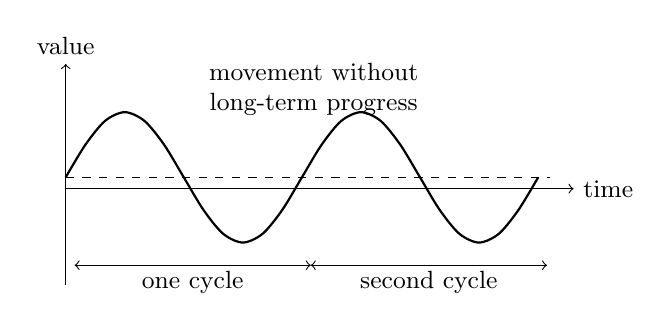
\begin{tikzpicture}[x=0.75cm,y=0.72cm, every node/.style={font=\small}]
\draw[->] (0,0) -- (8.6,0) node[right] {time};
\draw[->] (0,-1.7) -- (0,2.2) node[above] {value};
\draw[dashed] (0,0.2) -- (8.2,0.2);
\draw[domain=0:8,smooth,variable=\x,thick] plot ({\x},{1.15*sin(90*\x)+0.2});
\draw[<->] (0.15,-1.35) -- (4.15,-1.35);
\node at (2.15,-1.65) {one cycle};
\draw[<->] (4.15,-1.35) -- (8.15,-1.35);
\node at (6.15,-1.65) {second cycle};
\node[align=center] at (4.2,1.75) {movement without\\long-term progress};
\end{tikzpicture}
\end{adjustbox}
\end{center}

If two or more cycles merely produce a wave around a horizontal line, then there is no upward trend. There is only fluctuation. The investor who calls a short upward movement a trend is mistaking a fragment for the whole.

Reality does not move in straight lines. It moves in waves. From one point on a large wave, the nearby segment may look like a straight line, just as the ground beneath one's feet appears flat though the earth is curved. The shorter the view, the more easily a curve disguises itself as a line.

A useful rule follows:

\begin{quote}
Do not call a movement a trend until you have looked across at least two cycles.
\end{quote}

This rule is simple, but it protects the investor from many expensive illusions. Those who chase rises and cut losses in panic are often reacting to fragments. They do not see the cycle. They see only the latest slope.

\section*{Learning to Feel Gradual Change}

Most important changes are gradual before they become visible.

A child grows every day, yet the parent beside him may not notice. A relative who visits after many months sees the change immediately. The difference is not eyesight. The difference is distance from the gradient.

Investors, learners, and builders all need the ability to perceive gradual change. Without it, they overreact to sudden events and underreact to slow accumulation. They notice the news headline but miss the decade of preparation behind it. They notice the market crash but miss the long expansion before it. They notice the visible success but miss the quiet practice that made it possible.

This ability is not natural. It must be trained.

The best training method is recording.

Memory is too flexible to be trusted as a measuring instrument. It edits, compresses, excuses, exaggerates, and forgets. Records give the mind a firmer surface. They allow a person to compare today with a real earlier state rather than with a rewritten memory.

Record prices. Record decisions. Record reasons. Record attention spent. Record the state of a skill. Record the thesis behind an investment. Record the emotional condition under which a choice was made. Later, when the cycle has moved, the record becomes evidence.

\begin{center}
\begin{adjustbox}{max width=\linewidth}
\begin{tabular}{p{0.34\linewidth}p{0.5\linewidth}}
\hline
Without records & With records \\
\hline
Memory argues for comfort. & Evidence interrupts comfort. \\
Short movement feels decisive. & Cycles become visible. \\
Emotion rewrites the past. & Reasons can be inspected. \\
Mistakes repeat quietly. & Patterns can be corrected. \\
\hline
\end{tabular}
\end{adjustbox}
\end{center}

A person who records long enough begins to see what impatience cannot see: many ``sudden'' changes were only the public arrival of a long gradient.

\section*{The Harvestable Novice}

In some markets, the inexperienced speculator is compared to a crop that gets cut again and again. The image is crude, but the mechanism is accurate. A person becomes harvestable when he enters a market without homework, without cycle awareness, and without control over his own attention.

There are recognizable signs.

\begin{enumerate}
\item He asks whether a thing is ``reliable'' but cannot define the standard.
\item He asks whether something will rise, as if another person's confidence can replace his own work.
\item He treats a low nominal price as cheap and a high nominal price as expensive.
\item He feels unlucky whenever a buy is followed by a fall or a sale is followed by a rise.
\item He panics over ordinary fluctuation.
\item He celebrates paper gains as if they were permanent income.
\item He borrows confidence from the crowd, then blames the crowd when the result is bad.
\item He explains every outcome with luck, conspiracy, or betrayal.
\end{enumerate}

Most investors have had at least some of these thoughts. The point is not to feel superior. The point is to recognize the operating system that produces predictable loss.

One practical way to leave that state is to slow down trend judgment. Look across cycles. Ask what the movement means after a rise and a fall, not merely during the most exciting stretch. The market punishes people who live only in the latest candle, latest rumor, latest emotion, and latest price.

\section*{Rationalization}

Human beings are skilled at making their own behavior sound reasonable.

Even absurd behavior often has an internal explanation. The trader who has not studied cycles can still produce reasons. The person who refuses homework can say he is decisive. The person who chases a rise can say he is seizing opportunity. The person who sells in panic can say he is controlling risk. The person who refuses to learn can say the game is rigged.

The question is not whether a reason exists. A reason can almost always be found. The question is whether the reason survives inspection.

A useful self-check is:

\begin{quote}
Is this the result of thinking, or is it an excuse for avoiding thought?
\end{quote}

Progress often requires defeating one's own rationalization. This is uncomfortable because rationalization protects the current self. It allows the mind to avoid admitting laziness, fear, ignorance, envy, or impatience. But investment is too expensive a place to let rationalization remain in charge.

When someone else earns consistent returns, the lazy explanation is, ``He was lucky.'' Sometimes luck is involved. It would be foolish to deny that. But if one uses luck as a universal explanation, learning stops. A better question is, ``What did he understand, record, endure, or repeat that I did not?''

\section*{The Deeper Trend Behind Fluctuation}

Across long periods, asset classes reveal patterns that short periods hide.

Stocks can crash. Bonds can fall. Gold can rise for years and then stagnate. Currencies lose purchasing power slowly enough that many people notice only late. On a short chart, every asset can look dramatic. On a long chart, the question changes from ``What moved today?'' to ``What compounded across many cycles?''

The important lesson is not that one asset must always be chosen blindly. The lesson is that long-term trend and short-term volatility are different things.

\begin{center}
\begin{adjustbox}{max width=\linewidth}
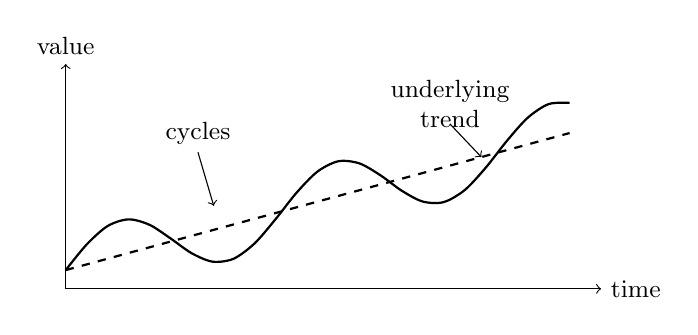
\begin{tikzpicture}[x=0.8cm,y=0.68cm, every node/.style={font=\small}]
\draw[->] (0,0) -- (8.5,0) node[right] {time};
\draw[->] (0,0) -- (0,4.2) node[above] {value};
\draw[domain=0:8,smooth,variable=\x,thick] plot ({\x},{0.35+0.32*\x+0.65*sin(105*\x)});
\draw[dashed, thick] (0,0.35) -- (8,2.91);
\node[align=center] at (2.1,2.9) {cycles};
\node[align=center] at (6.1,3.45) {underlying\\trend};
\draw[->] (2.1,2.55) -- (2.35,1.55);
\draw[->] (6.1,3.08) -- (6.6,2.46);
\end{tikzpicture}
\end{adjustbox}
\end{center}

A person who sees only the wave becomes emotional. A person who sees only the trend becomes careless. A competent investor sees both: the direction that may justify patience and the fluctuation that must be survived.

This applies to personal growth as well. Investing in one's own ability is likely to have a long-term upward trend, but the path is not smooth. There will be illness, confusion, bad teachers, poor projects, weak months, failed attempts, boredom, and delayed feedback. The person without cycle awareness interprets these as proof that the original decision was wrong. To ``cut losses,'' he abandons the very path that needed endurance.

This is how people become market novices outside the market. They buy high emotionally, sell low emotionally, and call it life planning.

\section*{Where Opportunity Hides}

Almost everything has cycles, but the cycles do not match.

A person's learning cycle, career cycle, family cycle, health cycle, cash-flow cycle, industry cycle, technology cycle, credit cycle, and market cycle may all be in different positions. This mismatch creates both opportunities and traps.

A good plan for one person at one time may be a bad plan for another person at another time. This is why life planning cannot be outsourced completely. Other people can provide models, questions, warnings, and examples. They cannot know the exact intersection of your cycles from the inside.

A simple map helps:

\begin{center}
\begin{adjustbox}{max width=\linewidth}
\begin{tabular}{p{0.28\linewidth}p{0.56\linewidth}}
\hline
Cycle & Question to ask \\
\hline
Personal cash flow & Can I hold through volatility without forced selling? \\
Learning cycle & Am I still acquiring the judgment required for this choice? \\
Industry cycle & Is the field expanding, maturing, or declining? \\
Market cycle & Is current emotion likely distorting price? \\
Life cycle & What obligations limit my risk capacity now? \\
\hline
\end{tabular}
\end{adjustbox}
\end{center}

Many failures occur not because the general idea was wrong, but because the investor's own cycle did not fit the action. A promising asset can still be a bad position if it forces sleeplessness, borrowing, panic, or family conflict. A good opportunity can be ruined by wrong sizing.

\section*{Calm Is Engineered}

Understanding cycles can change temperament.

What looks like persistence may simply be accurate location: the person knows where he is in the cycle and therefore does not interpret every decline as disaster. What looks like courage may be sizing: the person has arranged the position so that volatility cannot destroy him. What looks like patience may be cash flow: the person has other ways to earn money, so he does not demand that the investment provide immediate emotional comfort.

This matters because an investment that occupies too much of one's total assets becomes psychologically loud. For most ordinary people, if one position takes up a quarter of total wealth, complete calm is difficult. It is not useful to pretend otherwise. Overconfidence often begins with denying ordinary human limits.

The practical standard is plain:

\begin{quote}
I can remain well even if this money disappears.
\end{quote}

The amount that satisfies this condition differs by person. The way to increase it is not merely to become braver. It is to increase earning ability, reduce dependency, improve reserves, and build more than one source of income.

Here the biological lesson has an investment version: the more ways one can earn, the stronger the system becomes. Multiple earning methods allow invested capital to receive a longer sentence. It does not need to be released next week to pay for ordinary life. It can stay in the cell of time, where compounding has a chance to work.

If investment is the only way a person can earn, the mind becomes vulnerable. Every price movement feels personal. The eye moves from distant trend to nearby fluctuation. The investor becomes nearsighted and reactive. By contrast, a person with active earning power can give long-term capital the time it requires.

\section*{Bull Markets Still Hurt the Unprepared}

A beginner often imagines that a bull market makes everyone rich and a bear market makes everyone poor. Reality is not so clean.

Many people lose money in bull markets. They buy late, panic during ordinary pullbacks, sell at poor moments, then reenter with leverage because they cannot tolerate watching others make money. The rising environment does not save them from their own operating system.

Some people make money in bear markets. They have cash, patience, risk controls, and a thesis. They do not need every month to be pleasant. They understand that price and value can separate.

Market condition matters, but personal condition also matters. Without cycle awareness, a bull market can become a more efficient machine for transferring money away from the impulsive.

\section*{Technology Changes and the Death on the Road}

Large technological changes often create real long-term trends. They also create many deaths along the way.

The internet was real. Many internet investments still failed. Cloud computing was real long before the category became comfortable. Many early interpretations were wrong in timing, business model, or capital structure. The fact that a direction is correct does not mean every vehicle survives, every entry price is reasonable, or every investor can endure the cycle.

This is why trend judgment must be more precise than enthusiasm.

\begin{center}
\begin{adjustbox}{max width=\linewidth}
\begin{tikzpicture}[node distance=0.7cm, every node/.style={font=\small, align=center}]
\node[draw, rounded corners, minimum width=2.45cm, minimum height=0.75cm] (change) {real\\change};
\node[draw, rounded corners, minimum width=2.45cm, minimum height=0.75cm, right=of change] (hype) {public\\excitement};
\node[draw, rounded corners, minimum width=2.45cm, minimum height=0.75cm, right=of hype] (shake) {cycle\\shakeout};
\node[draw, rounded corners, minimum width=2.45cm, minimum height=0.75cm, right=of shake] (trend) {durable\\trend};
\draw[->] (change) -- (hype);
\draw[->] (hype) -- (shake);
\draw[->] (shake) -- (trend);
\end{tikzpicture}
\end{adjustbox}
\end{center}

The investor must ask: Is the change real? Which companies or assets actually capture the value? What cycle is the adoption process likely to pass through? How much capital can survive the shakeout? What evidence would prove the thesis wrong?

A trend is not a license to stop thinking. It is an invitation to think across time.

\section*{Prediction as Partial Vision}

Understanding cycles does not make anyone omniscient. No one sees the future completely.

But seeing a little more is still powerful. If one person sees nothing beyond today's price and another sees the current price inside a multi-year cycle, the difference compounds. If one person sees only discomfort and another sees discomfort as a known phase in learning, the difference compounds. If one person sees only temporary decline and another sees the underlying growth engine still functioning, the difference compounds.

Trend judgment is therefore not fortune-telling. It is disciplined partial vision.

A simple operating sequence is useful:

\begin{enumerate}
\item Define the object clearly. What exactly is being judged?
\item Identify at least one complete cycle: rise and fall, expansion and contraction, enthusiasm and disappointment.
\item Seek a second cycle or a comparable historical cycle.
\item Separate fluctuation from the underlying direction.
\item Record the judgment and the reasons before acting.
\item Size the action so that the cycle can be survived.
\item Review later with the original record, not with edited memory.
\end{enumerate}

This sequence does not guarantee profit. Nothing honest can. It does reduce the chance that emotion will dress itself as insight.

\section*{The Investor's Wider Practice}

Trend judgment belongs to the larger practice of wealth freedom.

Earlier chapters argued that attention is the most important personal asset, that capital has its own logic, that safety cannot be purchased by hiding from growth, that learning ability is a life lever, and that practice upgrades cognition. Cycle awareness connects these ideas.

Attention without cycle awareness becomes scattered by every fluctuation. Capital without cycle awareness becomes frightened money. Learning without cycle awareness becomes abandonment during the flat part. Practice without cycle awareness becomes discouragement before compounding appears. Hope without cycle awareness becomes fragile.

The mature practitioner learns to ask, again and again:

\begin{quote}
Which cycle am I in, and what trend is visible only beyond this cycle?
\end{quote}

This question creates calm because it creates distance. It also creates responsibility. If your life has multiple cycles, no outside expert can design it perfectly for you. You must learn, record, decide, act, and review.

The reward is not merely better investing. The reward is a more reliable world. The same events remain noisy, but the mind no longer treats all noise as signal. The same declines remain unpleasant, but they are no longer automatically interpreted as failure. The same opportunities remain uncertain, but uncertainty no longer forces paralysis.

To judge trends well is to become harder to harvest, harder to frighten, and harder to distract. It is to place the present inside a larger curve, then act according to the curve rather than according to the latest emotion.
